
%%%%%%%%%%%%%%%%%%%%%%% file typeinst.tex %%%%%%%%%%%%%%%%%%%%%%%%%
%
% This is the LaTeX source for the instructions to authors using
% the LaTeX document class 'llncs.cls' for contributions to
% the Lecture Notes in Computer Sciences series.
% http://www.springer.com/lncs       Springer Heidelberg 2006/05/04
%
% It may be used as a template for your own input - copy it
% to a new file with a new name and use it as the basis
% for your article.
%
% NB: the document class 'llncs' has its own and detailed documentation, see
% ftp://ftp.springer.de/data/pubftp/pub/tex/latex/llncs/latex2e/llncsdoc.pdf
%
%%%%%%%%%%%%%%%%%%%%%%%%%%%%%%%%%%%%%%%%%%%%%%%%%%%%%%%%%%%%%%%%%%%


\documentclass[runningheads,a4paper]{llncs2e/llncs}

\usepackage{amssymb}
\setcounter{tocdepth}{3}
\usepackage{graphicx}
%                   
\usepackage[pdftex,dvipsnames]{xcolor}  
\usepackage[colorinlistoftodos,prependcaption,textsize=tiny]{todonotes}
\newcommand\info[1]{\textcolor{red}{#1}}
%

\usepackage{url}
\urldef{\mailsa}\path|{bingbin.yu, jose.de_gea_fernandez, |  
\urldef{\mailsb}\path| yohannes.kassahun, vinzenz.bargsten}@dfki.de | 
%\urldef{\mailsc}\path|erika.siebert-cole, peter.strasser, lncs}@springer.com|    
\newcommand{\keywords}[1]{\par\addvspace\baselineskip
\noindent\keywordname\enspace\ignorespaces#1}

\begin{document}

\mainmatter  % start of an individual contribution

% first the title is needed
%\title{Modeling a SEA's Spring by using a data-driven method}
%\title{Learning the torque profile of a SEA's spring}
\title{Learning the Elasticity of a Series-Elastic Actuator for Accurate Torque Control }

% a short form should be given in case it is too long for the running head
%\titlerunning{Learning the torque profile of a SEA's springions}

% the name(s) of the author(s) follow(s) next
%
% NB: Chinese authors should write their first names(s) in front of
% their surnames. This ensures that the names appear correctly in
% the running heads and the author index.
%
\author{Bingbin Yu%
%\thanks{Please note that the LNCS Editorial assumes that all authors have used
%the western naming convention, with given names preceding surnames. This determines
%the structure of the names in the running heads and the author index.}%
\and Jos\'e de Gea Fern\'andez \and Yohannes Kassahun \and Vinzenz Bargsten}
%
\authorrunning{Lecture Notes in Computer Science: Authors' Instructions}
% (feature abused for this document to repeat the title also on left hand pages)

% the affiliations are given next; don't give your e-mail address
% unless you accept that it will be published
\institute{DFKI, Robotics Innovation Center,\\
Bremen, 28359, Germany\\
\mailsa\\
\mailsb\\
%\mailsc\\
}
%\url{http://www.springer.com/lncs}}

%
% NB: a more complex sample for affiliations and the mapping to the
% corresponding authors can be found in the file "llncs.dem"
% (search for the string "\mainmatter" where a contribution starts).
% "llncs.dem" accompanies the document class "llncs.cls".
%

\toctitle{Lecture Notes in Computer Science}
\tocauthor{Authors' Instructions}
\maketitle

\section{Abstract} 
Series elastic actuators (SEAs) have been frequently used in torque control mode by using the elastic element as torque measuring device. In order to precisely control the torque, an ideal torque source is critical for higher level control strategies. The elastic elements are traditionally  metal springs which are normally considered as linear elements in the control scheme. However, many elastic elements are not perfectly linear, especially for an elastic element built out of multiple springs or using special materials \cite{Rollinson2013}\cite{Paskarbeit2013} and thus their nonlinearities are very noticeable. %Besides the nonlinearities of the springs, the resistive frictions also effects the torque measurement
This paper presents two data-driven methods for learning the spring model of a series-elastic actuator: (1) a Dynamic Gaussian Mixture Model (DGMM) \cite{Edgington2009} is used to capture the relationship between actuator torque, velocity, spring deflection and its history. Once the DGMM is trained, the spring deflection can be estimated by using the conditional probability function which later is used for torque control. For comparison, (2) a deep-learning approach is also evaluated which uses the same variables as training data for learning the spring model. Results show that the data-driven methods improve the accuracy of the torque control as compared to traditional linear models. %These two approaches are evaluated with 
\keywords{series-elastic actuators, nonlinear springs, DGMM, deep learning, torque control}






%%%%%%%%%%%%%%%%%%%%%%%%%%%%%%%%%%%%%%%%%%%%%%%%%%%%%%%%%%%%%%%%%%%%%%%%%%%%%%%%%%%%%%%%%%%%%%%%%%%%%%%%%%%%%%%%%%%%%%%%%%%%%%%%%%%%%%%%%%%%%%%%%%%%%%%%%%%%%%%%%%%%%
\iffalse
Series elastic actuators (SEAs) have been frequently used for torque control by using the elastic elements in torque measurment. Traditionally, linear springs are adopted as the elastic element which are modelled with Hooke's law. In recent years, for improving the torque resolution, nonlinear springs (NLSs) are investigated as the elastic elements of SEAs \cite{Rollinson2013},\cite{Parietti2011},\cite{Paskarbeit2013}. In order to generate desired torque with NLSs, the corresponding deflection should be estimated, therefore a high-precision torque-deflection model is required. This paper presents a data-based method for modeling a NLS'torque-deflection of a SEA. The dynamic gaussian mixture model(DGMM) \cite{Edgington2009} is employed to capture the relationship between actuator torque, spring deflection, motor current and history of them. Once the DGMM is trained, the spring deflection can be estimated by using conditional probability function which later is used in torque control.
\fi
\iffalse
Rewrite:
\begin{itemize}
  \item Nonlinearity of the springs system exists in general(\cite{Kong2009}). Especially for the elastic element with multiple springs or with special material \cite{Rollinson2013}\cite{Paskarbeit2013}
  \item learning the torque profile means learning the spring nonlinearity and the resistive force which include static friction (backdrivability) and visous friction. The function of the model is similar to a observer.
%magnet torsional spring, paralle actuator
\end{itemize}
\fi


\section{Introduction}

In recent years, robots are increasingly developed to assist humans on direct physical interaction, not only in the field of %service
assistance and rehabilitation robotics \cite{Yu2013}, but also start to be used in industrial scenarios \cite{Rethink}. For these robots that work close to humans in  shared workspaces,  safety is of outmost concern (especially for industrial robots which normally are fast and powerful). To achieve a safe human-robot interaction, one possible solution is to use a compliant actuator that is able to immediately sense the torque and accommodate for external force disturbances. For a rigid actuator, the torque can be measured by torque sensors, e.g. a load cell, a strain gauge or a current sensor, and then be controlled by using a feedback loop \cite{Bargsten2016}. Different from a rigid actuator, a serial elastic actuator (SEA) can estimate the torque from the deflection of its elastic element. Due to the passive compliance between the actuator and its link, SEAs provide additional benefits including lower reflected inertia, greater shock tolerance and more accurate force control.\\

%In order to estimates the torque precisely with the elastic elements, an accurate torque-deflection model of the element is required. The elastic elements tranditionally are metal springs which are modelled by Hooke's Law.

A large number of SEA designs has already been developed, for instance as surveyed in \cite{Paine2014},\cite{Yu2013}. A typical design is a linear SEA, in which the spring system either uses a single spring \cite{Pratt1995} or a set of serial-connected springs \cite{Arumugom2009}, which connect to the motor through a ball screw.  For a rotary series elastic actuator (RSEA)  the design of the elastic coupling that restricts the size and reduces the weight of the device is usually challenging. For example, Kong and Jeon developed a compact RSEA with a coil spring and worm gears for knee joint assistance \cite{Kong2012}; Stienen et al. developed a rotational hydroelastic actuator with a symmetric torsion spring for a powered exoskeleton \cite{Stienen2010}; or the elastic element of the CAPIO actuator \cite{Mallwitz:2015} includes a set of small disc springs placed at both sides of a lever which connects to the link. In recent years, new elastic materials are also utilized: scientists at the Carnegie Mellon University used nonlinear rubber as the elastic element of the actuators for their snake robots \cite{Rollinson2013}; Sudano et al. integrated a magnetic nonlinear torsion spring in a rotary elastic actuator for biorobotic applications \cite{Sudano2014}. However, due to mechanical effects caused by the construction itself, by the structure of the spring system (e.g. different initial pre-compression of coil springs),  or the properties of the materials, many of these elastic couplings show very poor linearity, which is usually neglected. In this work, we propose two data-driven methods for modeling the torque profile of an SEA, which consider the nonlinearity of the elastic couplings for realizing better torque control approaches. The data-driven modeling methods are validated and compared using a newly designed RSEA. 

%A large number of SEA designs have already been developed, e.g. as surveyed in\cite{Paine2014},\cite{Yu2013}. A typical design is linear SEAs, the spring systems either use a single spring \cite{Pratt1995} or a set of serial-connected springs\cite{Arumugom2009} which connect to the motor through a ball screw (double check*). For a rotary series elastic actuator (RSEA), in order to limit the size and reduce the weight of the device, the design of the elastic coupling usually is more complicate. For example, Kong and Jeon developed a compact RSEA with a coil spring and worm gears for knee joint assistance\cite{Kong2012}; Stienen et al. developed a rotational hydroelastic actuator with a symmetric torsion spring for a powered exoskeleton\cite{Stienen2010}; the elastic element of CAPIO actuator\cite{Bargsten2016} which developed by DFKI GmbH includes a set of small disc springs placed at both sides of a lever which connects to the link. In recent years, new elastic materials are also utilized: scientists at the Carnegie Mellon University used nonlinear rubber as the elastic element of the actuators for their snake robots\cite{Rollinson2013}; ( the case of magnet coupling*).
%Due to mechanical effects/structure of the spring system (e.g. different initial pre-compressions of coil springs) or the property/characteristic of the material, many of these elastic couplings show poor linearities.


Various torque control approaches have already been proposed for SEAs, e.g. velocity-source control \cite{Wyeth2008}, a cascade control by using velocity or current in inner loop and torque in outer loop; or feedforward force control with disturbance observer \cite{Li2015}. The performances of these higher level control strategies are influenced by the torque sources, if the nonlinearity of the spring and resistive frictions are too large, a precise model of the elastic element and the frictions is needed. Therefore, Ford et al. \cite{Ford2014} proposed an online calibration method to compensate the nonlinear effects of the spring and accurately estimate the module’s output torque by using motor current and spring deflection together. Lu \cite{Lu2015} modelled the nonlinearity of the spring of a SEA by using a BP neural network and realized a stable velocity control. 
% cite paper : visco-elastic model from CMU
%, see \cite{Vallery2007}(cite a newer one*) for a survey
%(full paper not accessable yet)
The paper is organized as follows. In Section \ref{sec:SEAdesign}, the hardware design of the RSEA and analysis of the spring coupling are presented. In Section \ref{sec:ModelingMethods}, the two modeling methods of the elastic element are discussed. The experimental validation of the two models is performed in Section \ref{sec:ModelValidation}. %where the velocity effects are not considered.
In Section \ref{sec:TorqueControl}, based on the learned models, a torque control task is demonstrated. Finally, conclusions are given in Section \ref{sec:Conclusion}.






%%%%%%%%%%%%%%%%%%%%%%%%%%%%%%%%%%%%%%%%%%%%%%%%%%%%%%%%%%%%%%%%%%%%%%%%%%%%%%%%%
%Various torque control approaches have already been proposed for SEAs, e.g. velocity-source control \cite{Wyeth2008}, a cascade control by using velocity, current in inner closed loop and torque in outer loop;  feedforward force control with disturbance observer\cite{Li2015} %or.. . 
%For a nonlinear SEA, the nonlinearity of the elastic element should also be compensated together with the other nonlinear effects of the system, such as the friction, stiction, backlash and reflected inertia in the gear train. %(backlash and reflected inertia in the gear train.?)


% cite paper 3: 'Control of Robots with Elastic Joints based on Automatic Generation of Inverse Dynamics Models' Michael Th¨ummel, Martin Otter and Johann Bals
% cite paper 4: 'Demonstrating the Safety and Performance of a Velocity Sourced Series Elastic Actuator' Gordon Wyeth, Member, IEEE
% cite paper 5: "Design and Control Considerations for High-Performance Series Elastic Actuators"




%then a pure high-gain PID approach can suffer from stability issues.
%For a nonlinear SEA, the nonlinearity of the elastic element should also be compensated together with the other nonlinear effects of the system, such as the friction, stiction, backlash and reflected inertia in the gear train. %(backlash and reflected inertia in the gear train.?)

%\todo[inline]{\small Introduction points:}

%1)(comparing to rigid actuator) elastic actuator is better in initial touch of human-robot interaction and provides a cheap torque sensing.
%2)linear spring model and non-linear spring model.
%3)torque control method:  compare "torque-spring model+deflection control" to the other approaches. }
%However,   current   SEA   designs   face   a   common   performance  limitation  due  to  the  compromise  on  the  spring  stiffness selection.
%magnet torsional spring, paralle actuator

%\cite{Yu2015} \cite{Austin2015}?

%However,   current   SEA   designs   face   a   common    performance  limitation  due  to  the  compromise  on  the  spring   stiffness selection.

%An ideal force source is the common building block for several higher level control strategies, including: operational space control, virtual model control, impedance control, and classical model-based control, among others. In this paper, we only consider classical model-based position control as an extension to a near-ideal force source. We create this near-ideal force source by developing a force control strategy which attempts to minimize measured force error by 

%which takes an input of motor current and produces spring deflection as an observable output. 

%The ideal force mode implies that: 1) the actuator has (output shaft) zero impedance so that it is perfectly back-drivable; and 2) the force (torque) output is exactly proportional to the controlinput.

%In general, a spring is a nonlinear element, i.e., the spring force is a nonlinear function of the spring deflection






\section{SEA design and spring analysis}
\label{sec:SEAdesign}
The assembled serial elastic actuator (see Fig. \ref{fig:4by3_50Nm_actuator} left) is designed within the project FourByThree \cite{Jose2016}. The actuator is powered by a Robodrive brushless DC motor and provides a maximum 50 Nm torque and 15 rpm speed in the link side by using a 1:120 Harmonic Drive gear. An FPGA (Spartan6)-based control stack  incorporates all the required sensors (three absolute encoders, two motor current sensors, temperature sensors, etc.) and perform the required actuator control with an in-house developed communication protocol (Node-level Data Link Communication (NDLCom \cite{Zenzes2016})). A new elastic element based on coil springs has been developed for the actuator (Figure \ref{fig:4by3_50Nm_actuator} right) which consists two springs in each spring segment: a lower-stiff spring firstly compresses singly until its deflection reaches approx. 5 degree, then a smaller higher-stiff spring which is placed inside the other starts to work. By using this design, the elastic spring is relatively `soft' in the lower torque range, so that it provides a higher torque to deflection resolution in this torque range. Since the elastic spring is `stiff' for a higher torque input, it brings a larger working range and avoid that the spring completely compresses at the maximum torque. 

%%%%%%%%%%%%%%  Figure: elastic motor and spring 50Nm   %%%%%%%%%%%%%%%%%%%%%%%%%
\begin{figure}[htb]
\centering
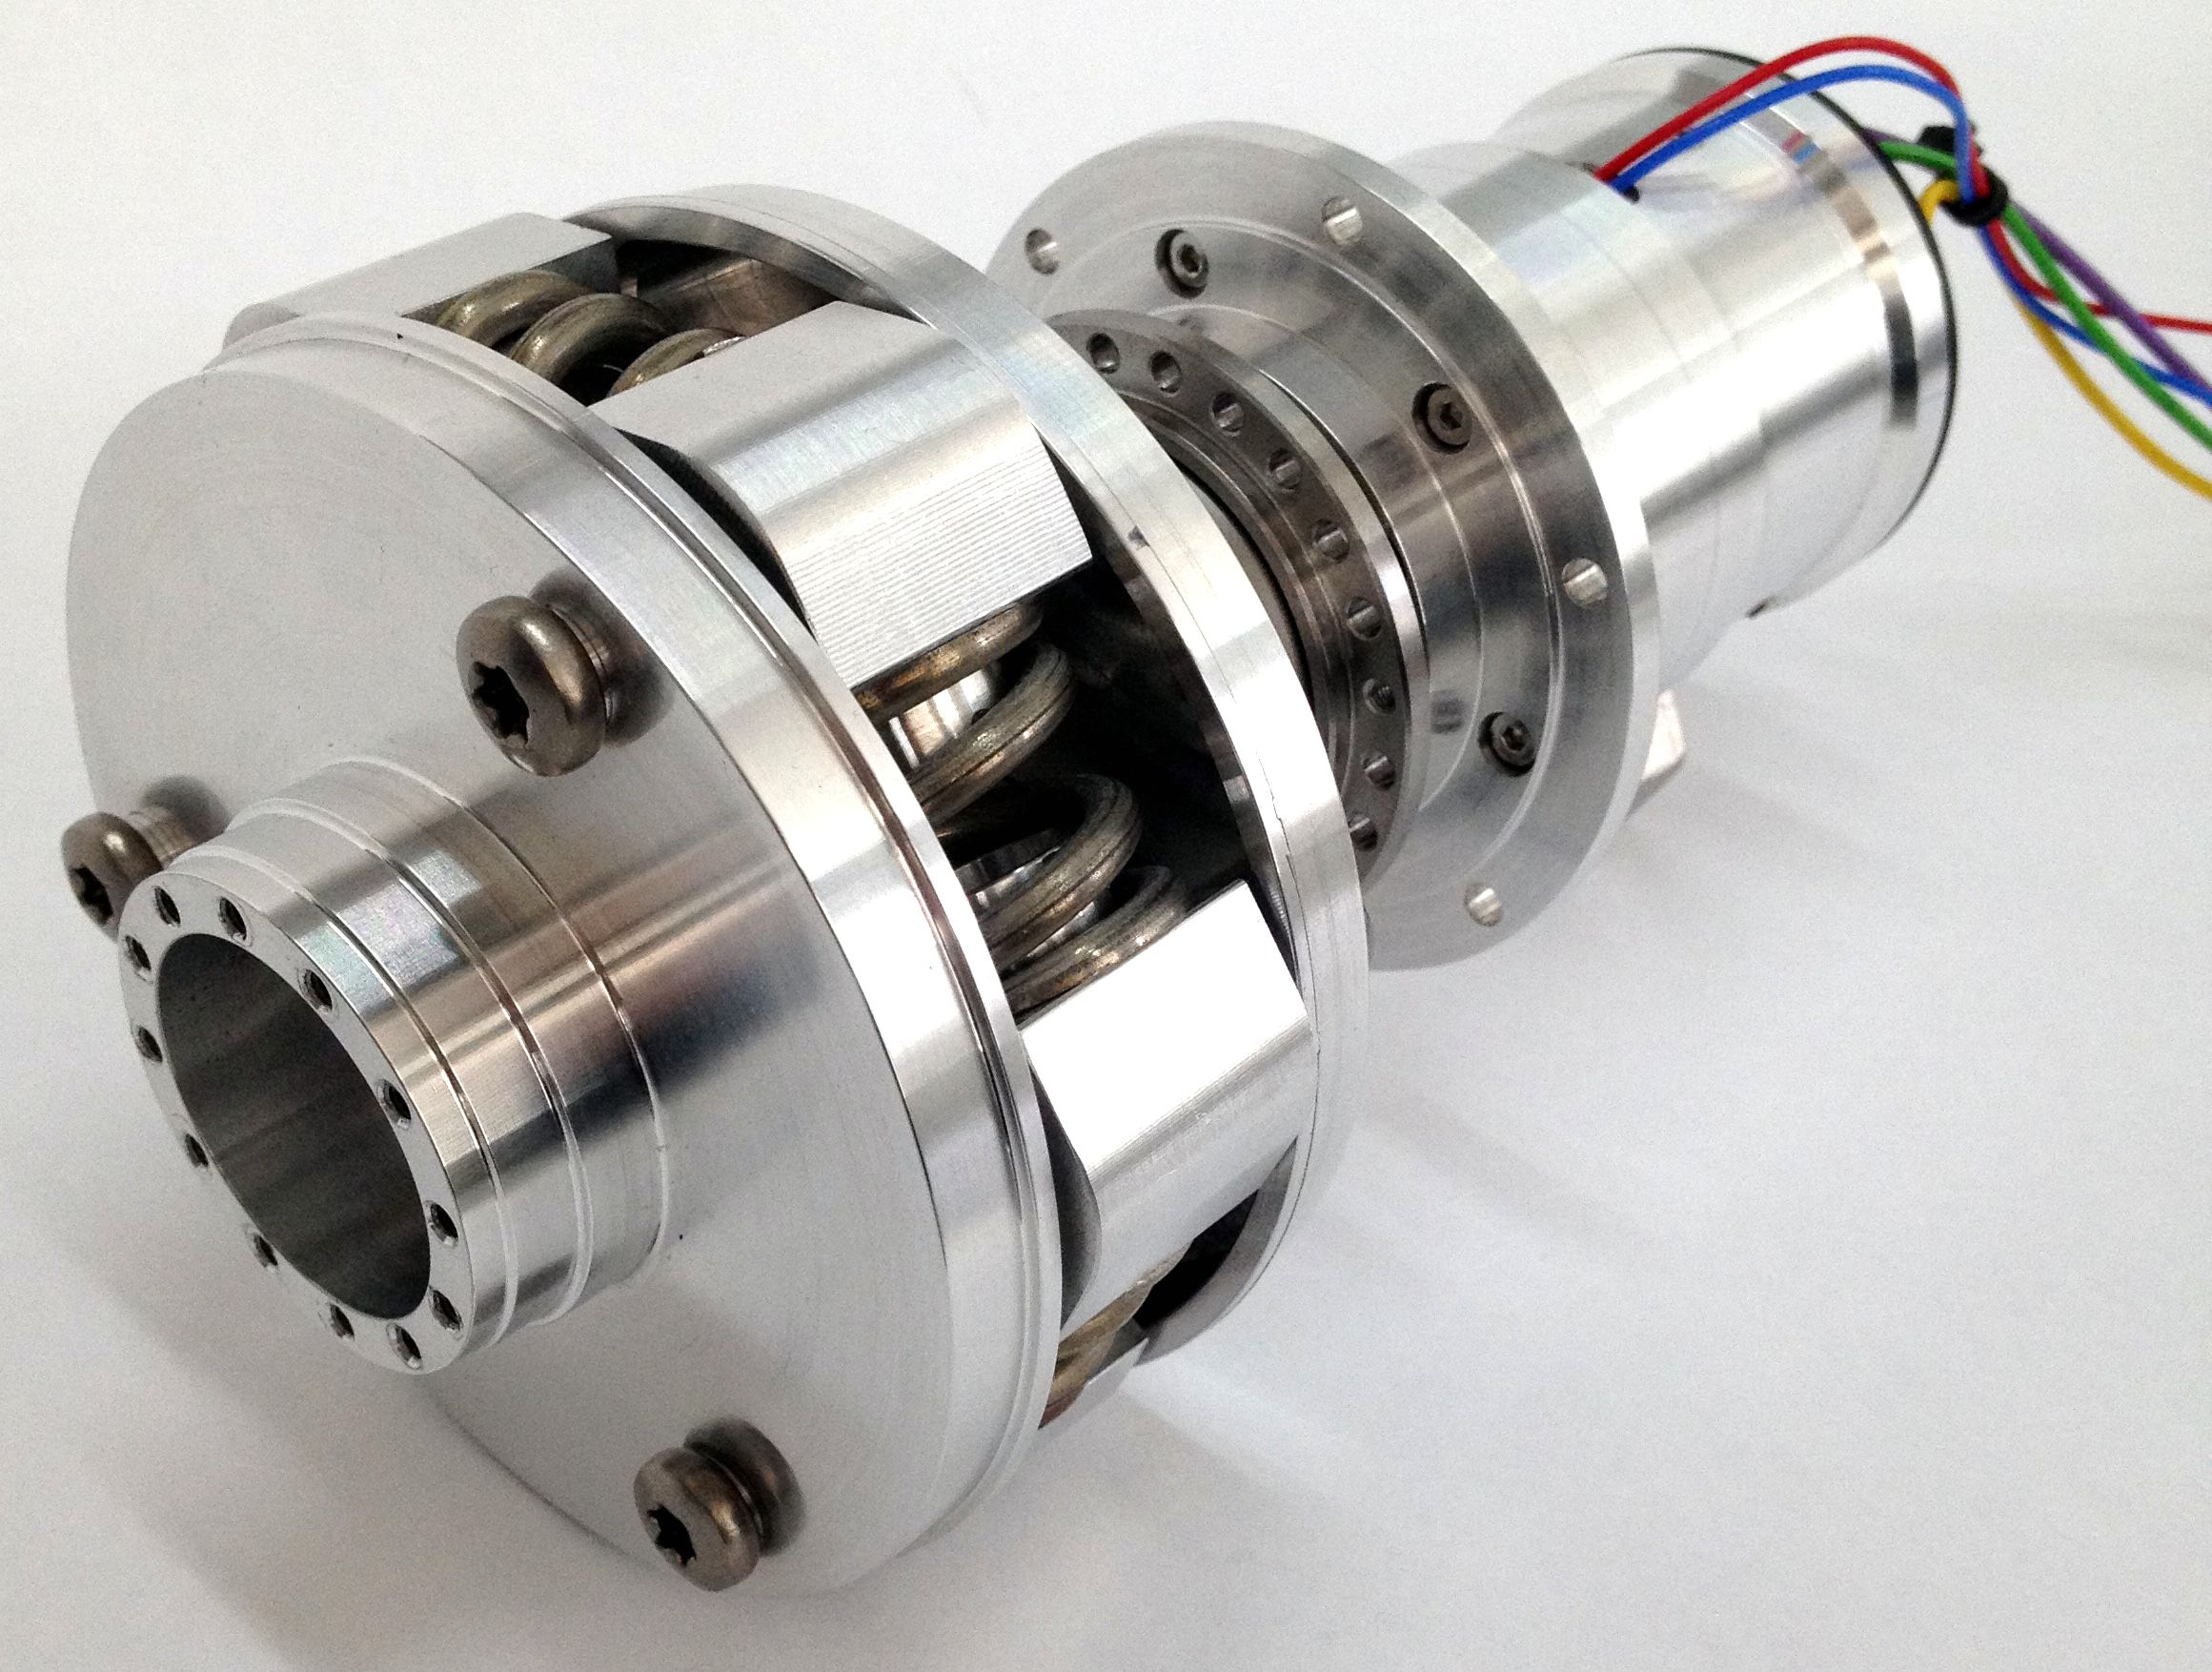
\includegraphics[width=0.4\columnwidth]{./images/50NmJoint_WithoutHousing_07.jpg}
%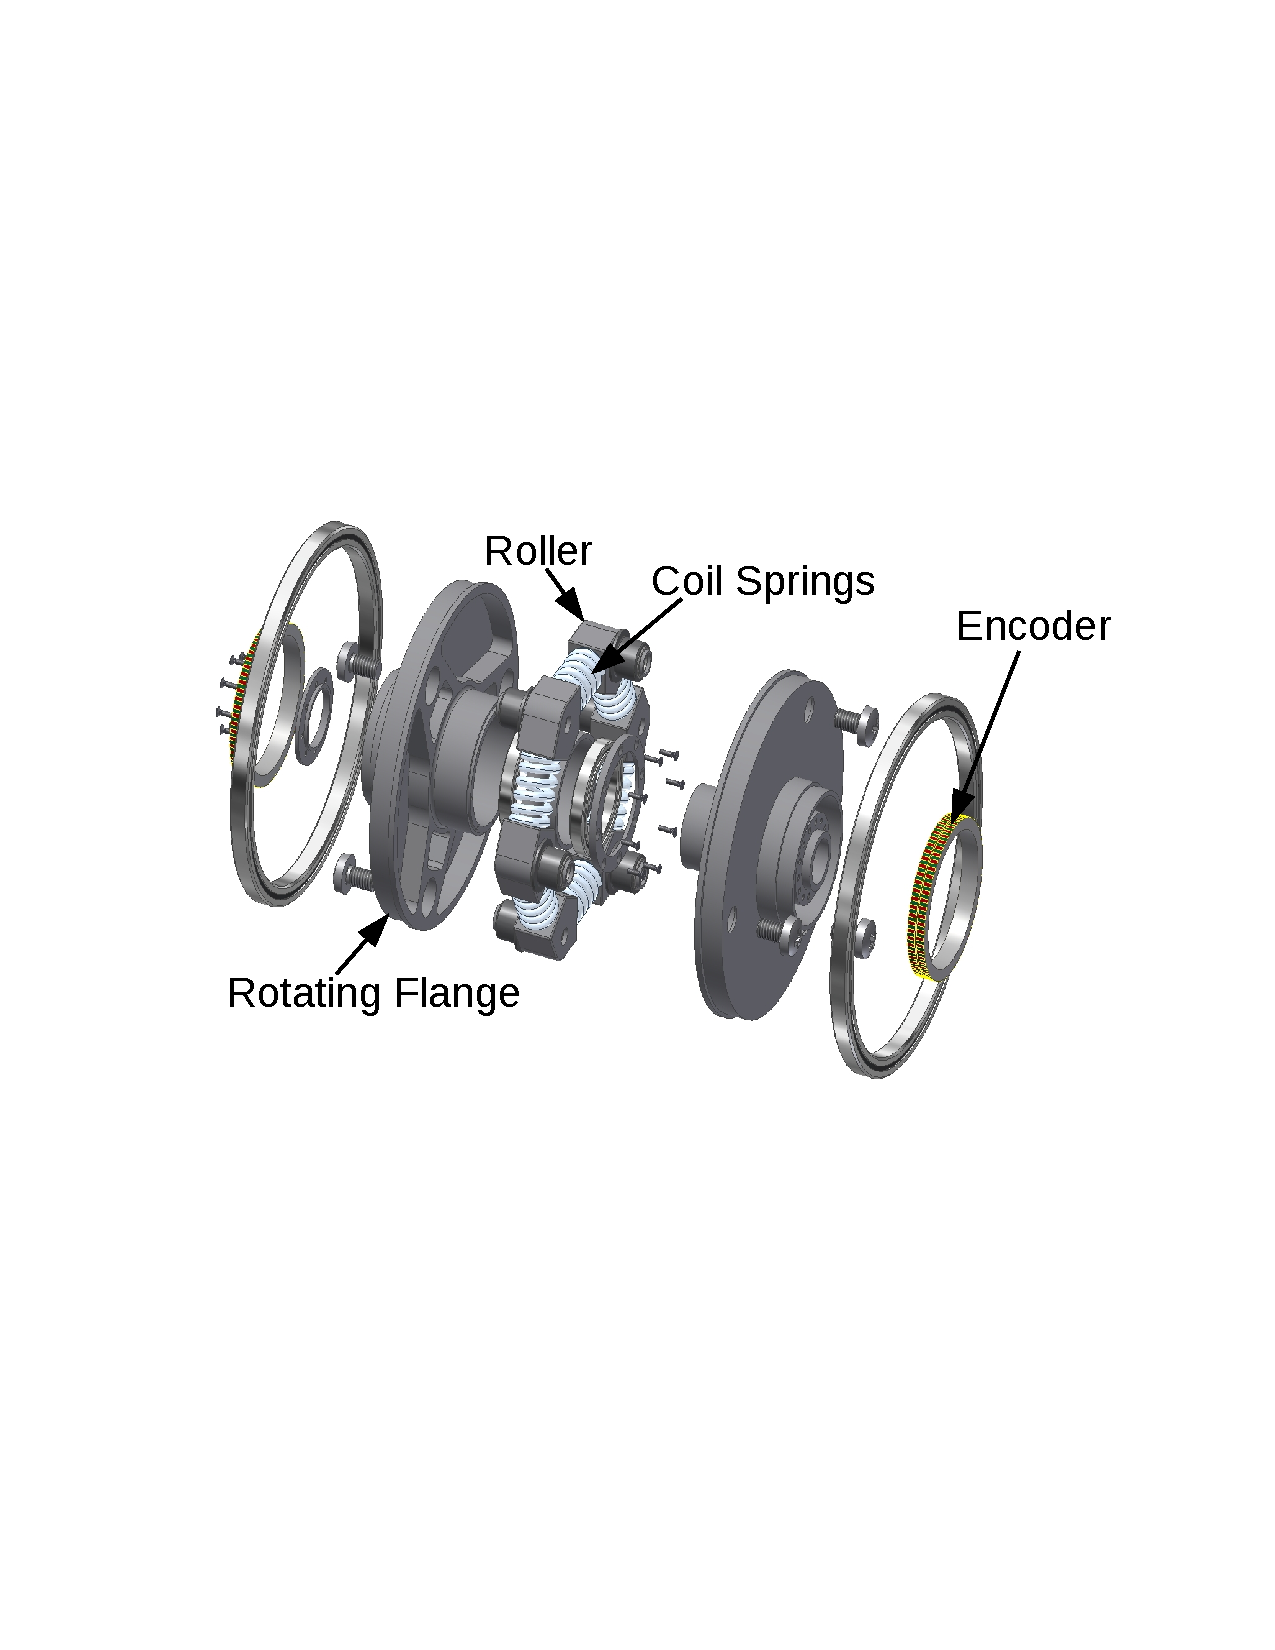
\includegraphics[clip, trim=2.5cm 9.5cm 2.5cm 8.5cm,width=0.5\columnwidth]{./images/Spring_coupling_structure.pdf}
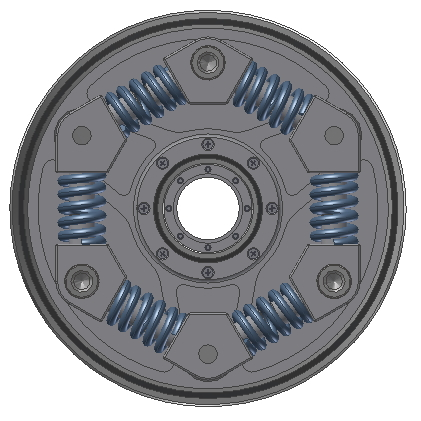
\includegraphics[width=0.3\columnwidth]{./images/Spring_Coupling_03.jpg}
 \caption{\textit{left:} FourByThree 50Nm-Actuator. \textit{right:} Elastic element based on coil springs.}
 \label{fig:4by3_50Nm_actuator}
\end{figure}
%%%%%%%%%%%%%%%%%%%%%%%%%%%%%%%%%%%%%%%%%%%%%%%%%%%%%%%%%%%%%%%%%%%%%%%%%%%%%%%

As shown in Figure \ref{fig:4by3_50Nm_actuator},  coil springs are used and each single spring is a linear element. However due to the internal friction and different pre-compression during assembly, the torque-deflection curve of the overall spring module is nonlinear. Figure~\ref{fig:Spring_torque_curve_2D} shows the result of an experiment used to demonstrate the nonlinearity of the spring coupling. In this experiment, the elastic actuator is controlled to a fixed rotation angle in position control. An external force/torque sensor (Lorenz-DF30) is employed to provide a torque ground truth in a range of -50Nm to +50Nm with an accuracy class of 0.05\%.  The motor is fixed on a test bed, the external torque is externally applied to the spring through the link lever in both directions. As the plot shows, the torque-deflection model of the spring presents a hysteresis characteristic, where a simple linear regression line is a poor choice of representation.

%%%%%%%%%%%%%%  Figure: static analysis of the spring coupling  %%%%%%%%%%%%%%%%%%%%%%%%% 
\begin{figure}[htb]
\centering
\advance\leftskip 0.3cm
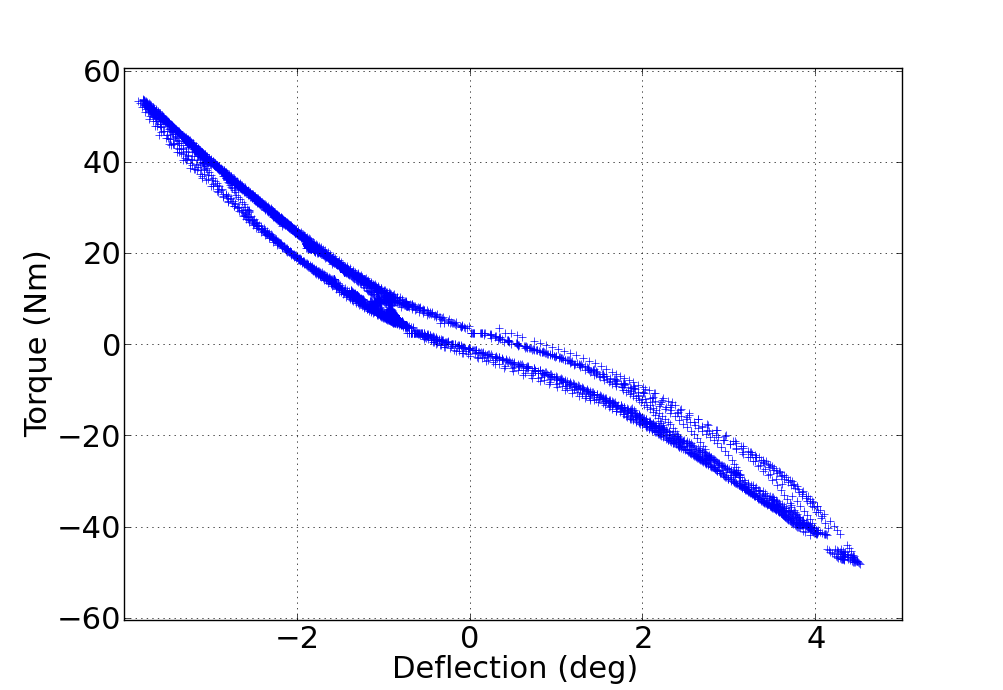
\includegraphics[width=0.9\columnwidth]{./images/spring_static_analysis.png}
 \caption{Torque to deflection curve of the spring coupling. The output torque is measured with an external force/torque sensor and the deflection is measured by computing the difference of two absolute encoders at both sides of the spring.}
 \label{fig:Spring_torque_curve_2D}
\end{figure}
%%%%%%%%%%%%%%%%%%%%%%%%%%%%%%%%%%%%%%%%%%%%%%%%%%%%%%%%%%%%%%%%%%%%%%%%%%%%%%%

% Following sections will be updated with new results
\section{Spring modeling methods}
\label{sec:ModelingMethods}
Since a spring is used as a torque sensor in a series-elastic actuator, an accurate spring model is the basis of a successful and accurate torque control. As discussed in Section \ref{sec:SEAdesign}, the torque-deflection curve of the coil spring component exhibits a nonlinear property. In order to account for the nonlinearity, two data-driven modeling approaches are used: a dynamic Gaussian mixture model (DGMM) and (2) a neural network. Both methods will be described briefly in the following sections.


\subsection{Spring modeling by DGMM}
 As a probabilistic modeling method, Gaussian mixture models (GMM) \cite{Edgington2009} are widely used in modeling complex and multi-variable data. To model the spring with more variables besides deflection, a dynamic Gaussian mixture model (DGMM) is studied, which represents a probability density function $P(x)$ as a variable-sized set of “weighted Gaussian” pairs (Eq.~\ref{eq:dgmm1}).
\iffalse
\begin{equation}
    G={(g_{1}(x),\omega_{1})+(g_{2}(x),\omega_{2})+......(g_{m}(x),\omega_{m})},
 \label{eq:dgmm1}
\end{equation} 
\fi
\begin{equation}
    P(x)=\Sigma_{i=1}^{m}\hat{\omega_{i}}g_{i}(x),
 \label{eq:dgmm1}
\end{equation} where $g_{i}(x)$ is a multivariate Gaussian distribution 

\begin{equation}
    g_{i}(x)=p_{i}(x) \sim \mathcal{N}_{i}(\mu_{i},\Sigma_{i}),
 \label{eq:dgmm2}
\end{equation} and $\hat{\omega_{i}}$ is the weight of the Gaussian $g_{i}(x)$

\begin{equation}
    \hat{\omega_{i}}=\omega_{i}/\Sigma_{k=1}^{m}.
 \label{eq:dgmm3}
\end{equation} The quantity $x$ is the observation vector. As Figure~\ref{fig:4by3_50Nm_actuator} shows, the torque to deflection curve of the spring coupling is nonlinear, therefore more variables are required: the rotation velocity $v$ and the history of the spring deflection $\delta^{\prime}$. Consequently, the observation vector is

\begin{equation}
    x=[\tau,\delta,\delta^{\prime},v],
 \label{eq:dgmm4}
\end{equation} and the model of the system can be represented by

\begin{equation}
    P[\tau,\delta,\delta^{\prime},v].
 \label{eq:dgmm5}
\end{equation} As a result, once a DGMM model $P[\tau,\delta,\delta^{\prime},v]$ is learned with a training data set, the output torque can be estimated analytically as

\begin{equation}
	\mathbb{E}[\tau|\delta, \delta^{\prime}, v].
 \label{eq:dgmm9}
\end{equation} For control purposes one can also similarly estimate the deflection using

\begin{equation}
	\mathbb{E}[\delta|\tau, \delta^{\prime}, v].
 \label{eq:dgmm10}
\end{equation}

%The conditional mean for Gaussian $g_{i}$ is a linear function given by
%\begin{equation}
%	m_{i}(z)=E_{i}[Y|Z=z]=\mu_{i}^{z}+\Sigma_{i=1}^{YZ}(\Sigma_{i=1}^{ZZ})^{-1}(z-\mu_{i}^{z}),
% \label{eq:dgmm6}
%\end{equation} 

%$\mu_{i}$ is the mean Gaussian $g_{i}$, then the conditional mean can be calculated by:

%\begin{equation}
%	E[Y|Z=z]=\Sigma_{i=1}^{m}\pi_{i}(z)m_{i}(z),
% \label{eq:dgmm7}
%\end{equation} 
%where

%\begin{equation}
%	\pi_{i}(z)=\frac{\hat{\omega_{i}}\mathcal{N}(z;\mu_{i},\Sigma_{i})}{\Sigma_{k=1}^{m}\hat{\omega_{k}}\mathcal{N}(z;\mu_{k},\Sigma_{k})}.
% \label{eq:dgmm8}
%\end{equation} 

\subsection{Spring modeling by using neural network}

An artificial neural network consists of an interconnected assembly of simple processing units \cite{Bishop1995}. In most of the cases, each processing unit calculates its output by taking a weighted sum of its inputs and transforming the sum by an activation function. In addition to the connection weights, the function represented by an artificial neural network is determined by the architecture of the neural network. Because of the possibility of optimizing a large number of parameters due to the advancement in computing, neural networks are used in various application areas such as computer vision, reinforcement learning, speech recognition and natural language processing resulting in progress beyond the state-of-the-art in terms of performance in most of the cases.

In this paper, three layered neural networks with relu activation function are used for modeling the functions $\mathbb{E}[\tau|\delta, \delta^{\prime}, v]$ and $\mathbb{E}[\delta|\tau, \delta^{\prime}, v]$. A relu (rectifier function) is defined as $ f(a) = \max(0,a)$, where $a$ is a weighted sum of the inputs to a unit. Unlike DGMM, two separate networks are trained independently: once for $\mathbb{E}[\tau|\delta, \delta^{\prime}, v]$ and once for $\mathbb{E}[\delta|\tau, \delta^{\prime}, v]$. The neural networks are realized and trained using the open-source Deep Learning tool Keras \cite {Keras}. \info{some details about the exact structure of the NN? layers... input dimension...and so on...}
















\section{Spring models validation}
\label{sec:ModelValidation}

In order to validate the two modeling approaches, an experiment setup has been constructed as shown Figure~\ref{fig:Spring_torque_exp_setup}. The FourByThree 50 Nm SEA (for more details, see Section \ref{sec:SEAdesign}) is used and fixed on an adjustable base, so that the inclination of the actuator can be changed and the effects of gravity can be accounted for. An external force/torque sensor is mounted between the spring coupling and the link lever, which measures the output torque with a 125 Hz sampling frequency in order to validate the results.

%%%%%%%%%%%%%%%%%%%%     Figure: testbed      %%%%%%%%%%%%%%%%%%%%%%%%
\begin{figure}[htb]
\centering
\advance\leftskip 1.5cm
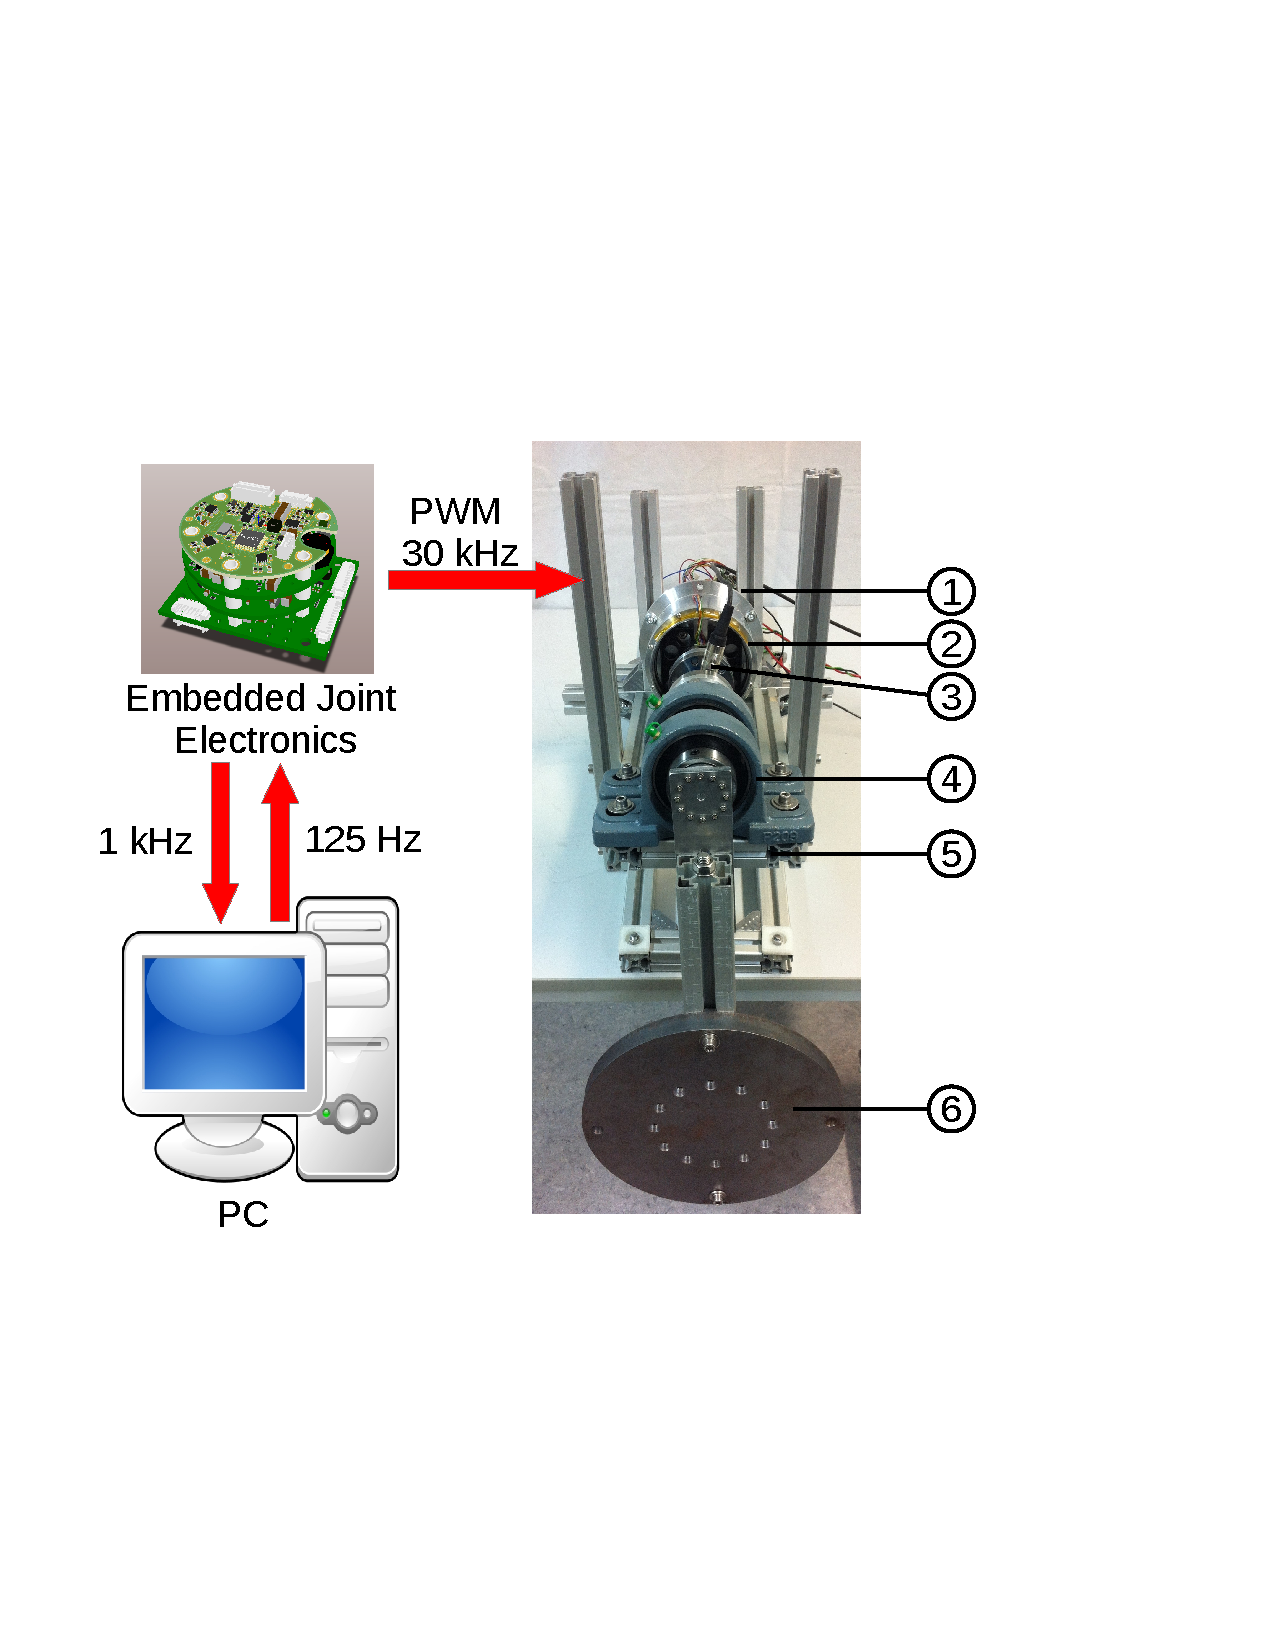
\includegraphics[clip, trim=0.5cm 7cm 0.5cm 7.5cm,width=0.88\columnwidth]{./images/4by3_springmodel_testbed.pdf} 
 \caption{Experimental setup used for spring modeling and torque control: 1) actuator; 2) spring coupling; 3) external force/torque sensor; 4) brake; 5) adjustable base; 6) load.}
 \label{fig:Spring_torque_exp_setup}
\end{figure}
%%%%%%%%%%%%%%%%%%%%%%%%%%%%%%%%%%%%%%%%%%%%%%%%%%%%%%%%%%%%%%%%%%%%%%%

The models need to be trained first and then be used in the validation phase by estimating the output torque given measured variables. In the training procedure, the inclination angle of the actuator base is set to 0 degree and the training data is gathered by controlling the load to rotate in the range of approx. $\pm170$ degrees with position control smoothly in a very low speed. %Since the load velocity and acceleration are approaching to zero, the velocity related dynamic effects can be neglected.  %Therefore, the nonlinearity of the spring coupling and the static friction are modelled in this experiment. 
The position of the load at the link lever is changed in each train test and the actuator torque $\tau$, deflection $\delta$, first derivative of deflection $\delta^{\prime}$ and velocity $v$ are measured as the training inputs. The spring deflection is extracted from two absolute encoders, the first derivative of deflection $\delta^{\prime}$ is calculated from the change of the deflection and the time used in a control cycle and the velocity $v$ is acquired from the position sensor. 

In the validation phase, the same load is fixed at random selected position on the lever arm and the inclination angle of the base is set to 37.8 degree. %Therefore, the data which gathered from testing experiment is different to the training data.
Based on the trained DGMM and neural network models, the actuator torque $\tau$ can be estimated by both methods respectively. Figure \ref{fig:springmodelcomparison} shows the comparison results between the trained DGMM model $P[\tau,\delta,\delta^{\prime},v]$, the neural network model, and the linear regression model.

%%%%%%%%%%%%%%%%%%%%  Figure: model comparison %%%%%%%%%%%%%%%%%%%%%%%%
\begin{figure}[htb]
\centering
\advance\leftskip-1.2cm
%\hspace*{-1.5in}
%\vspace*{-1.1 cm}
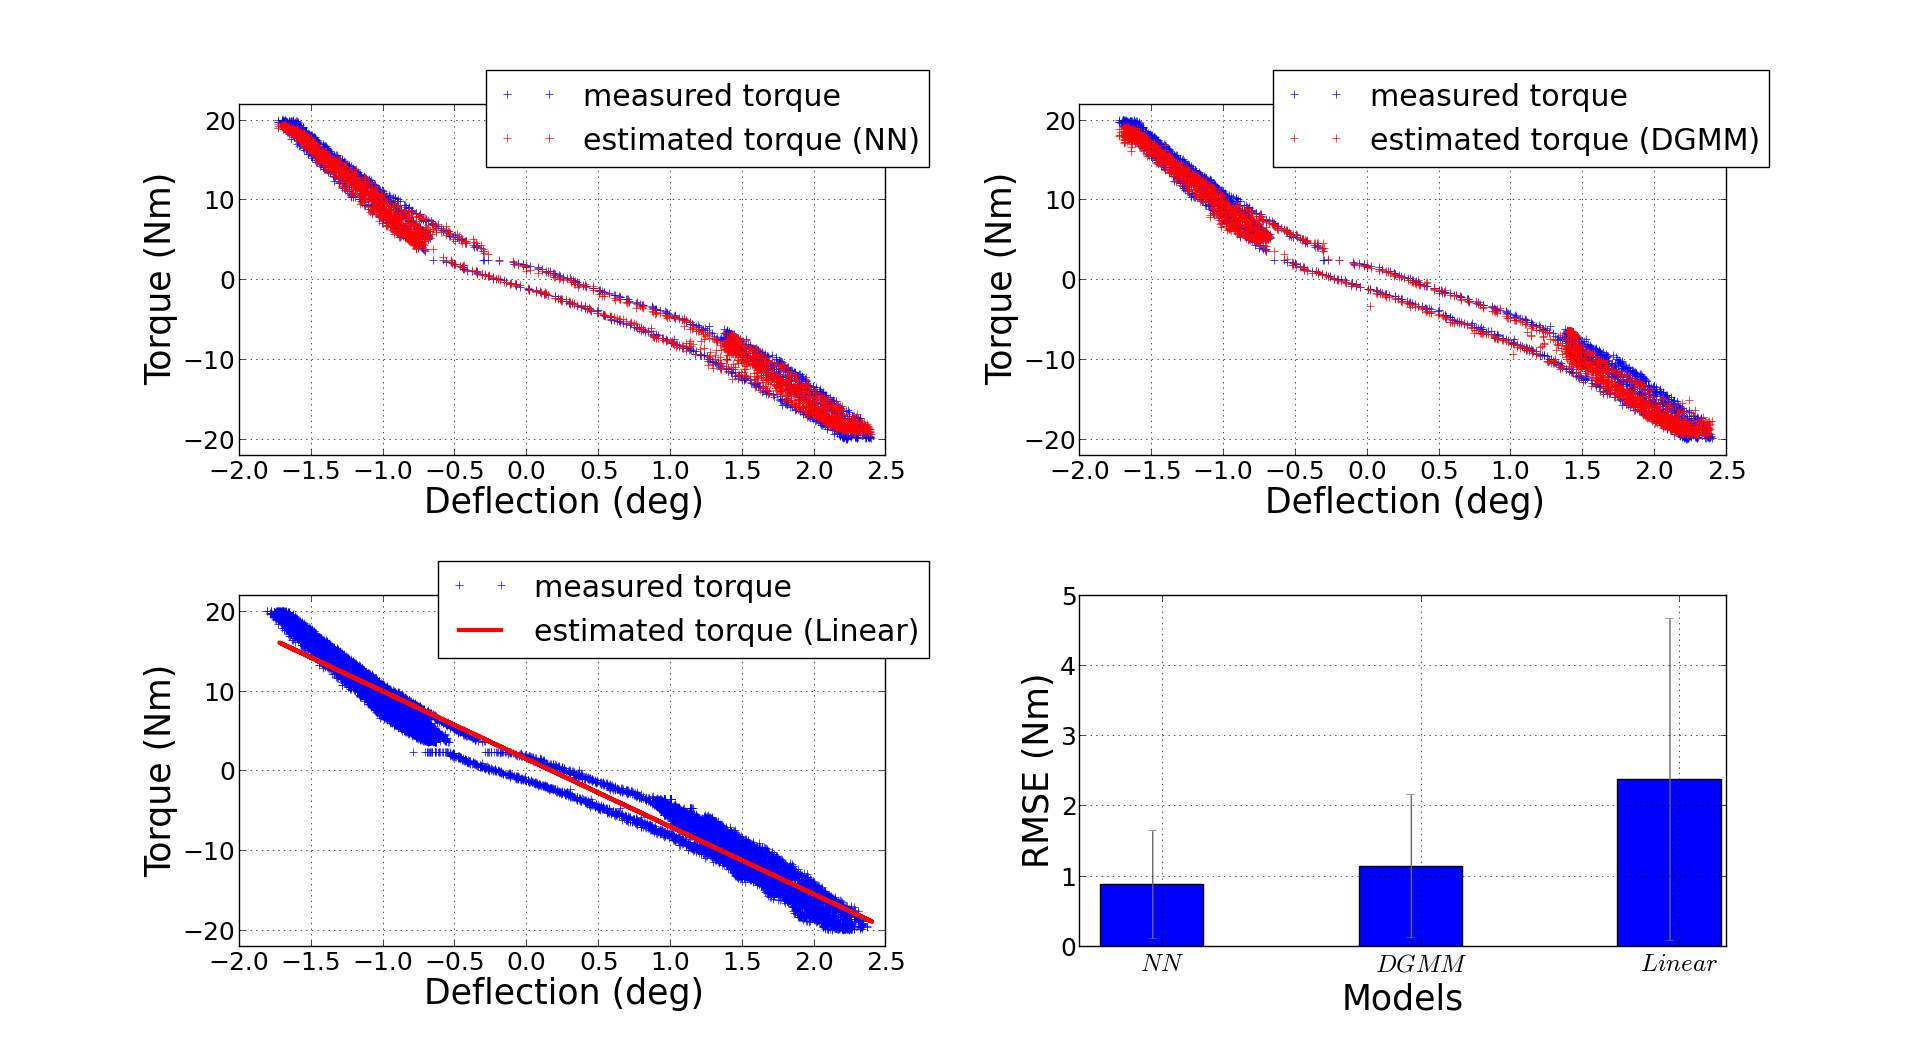
\includegraphics[width=1.22\columnwidth]{./images/4by3_model_comparison_new.png}
 \caption{\textit{Upper left:} measured torque-deflection curve (blue crosses) and estimated torque with neural network model (red crosses). \textit{Upper right:} measured torque-deflection curves (blue crosses) and estimated torque with DGMM model (red crosses), \textit{lower left:} measured torque-deflection curve (blue crosses) and corresponding fitted linear line (red line), \textit{lower right:} root mean square errors (blue bars) and normalized standard deviations (black line) of the three models in torque estimation.}
 \label{fig:springmodelcomparison}
\end{figure}
%%%%%%%%%%%%%%%%%%%%%%%%%%%%%%%%%%%%%%%%%%%%%%%%%%%%%%%%%%%%%%%%%%%%%%%

As can be seen from the upper left and upper right plots, both DGMM and neural network models are able to predict the output torque given the measured variables with high accuracy. In contrast, the fitted linear regression function has problems to represent the torque-deflection curve (see lower left plot). The RMSE between the estimated torque and measured torque is calculated for each model, as the lower right plot shows; the DGMM and neural network models present a comparable performances and have a large advantage compared to the linear model.




\section{Torque control}
\label{sec:TorqueControl}
Based on the learned spring models, a torque controller is proposed to control the spring torque to track the desired torque as precisely as possible. The complete torque control scheme of the SEA consists of three cascaded control loops for motor current, spring deflection and torque (see Fig. \ref{fig:controller_structure}). %An inner current loop is used to control the brushless DC motor in the PWM. 
Two absolute encoders are installed at both sides of the spring coupling for measuring the rotation angle and calculate the spring deflection. A deflection PID controller is implemented into the FPGA which closes the loop with the spring deflection and then cascades with an inner motor current controller. The first derivative of the deflection and the velocity are calculated to be used as the inputs of the spring model, together with the given desired torque, and the corresponding deflection value is estimated. This deflection will be then controlled by the inner deflection and current controllers. Due to an intrinsic property of the DGMM model, once the model $P[\tau,\delta,\delta^{\prime},v]$ is learned from the training experiments, both forward $E[\tau|\delta, \delta^{\prime}, v]$ and inverse models $E[\delta|\tau, \delta^{\prime}, v]$ can be estimated, whereas the inverse model is then used in the torque control. In contrast, the forward and inverse models need to be trained individually when using a neural network model.


%In addition, a joint position and velocity controller are working in the background. They are activated only in case a set limit of velocity or position is reached and then override the deflection controller.
%%%%%%%%%%%%%%%%%%%%  Figure: control structure   %%%%%%%%%%%%%%%%%%%%%%%%%%%
\begin{figure}[htb!]
    \centering
    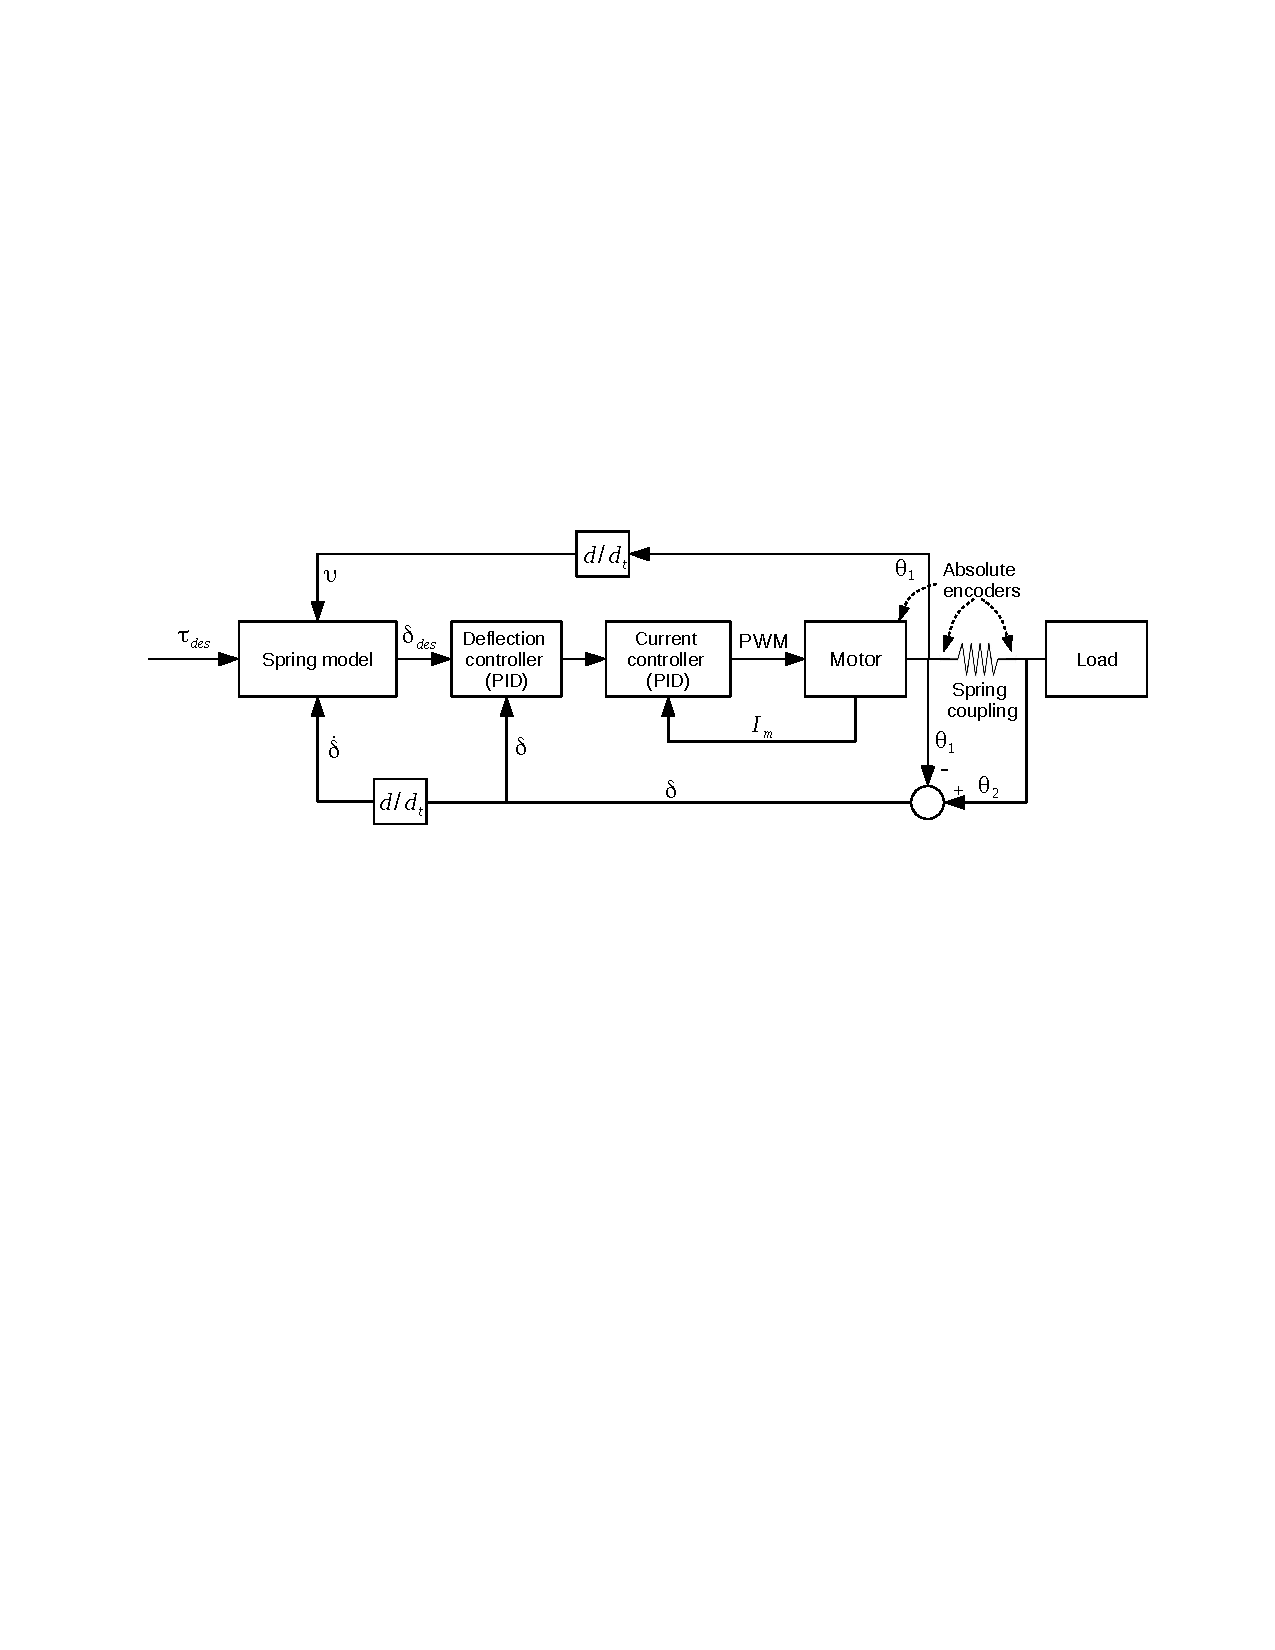
\includegraphics[width=1\textwidth, trim=2.5cm 13cm 2cm 8.5cm, clip]{images/torque_control_block_diagram.pdf}
    \caption{Complete actuator torque control scheme}
 \label{fig:controller_structure}
\end{figure}
%%%%%%%%%%%%%%%%%%%%%%%%%%%%%%%%%%%%%%%%%%%%%%%%%%%%%%%%%%%%%%%%%%%%%%%%%%%%%
The proposed torque control is verified in two torque tracking experiments. A chirp signal and a random-walk are given as the desired torques in these two experiments respectively (green lines) and the different controllers which are based on different spring models are evaluated in measured output torques (red and blue lines, see plot a,b of Fig.~\ref{fig:torque_tracking_result}). As can be seen from the comparison in tracking errors (see plot c,d), the torque control by using DGMM model presents better results than by using linear model in both experiments. Since the viscous friction of the system can not be compensated by the spring models completely, the performance of random-walk tracking (rmse=0.90) is better than chirp tracking (rmse=1.13), and the error of the chirp tracking is also raised slightly when the reference frequency is increased. 

%In the experiment of tracking a random-walk signal, since the output torque is controlled to follow step singals, the load approaches static when the given torque is constant. Therefore, the viscous friction which needs to be compensated is lower than that in the experiment of chirp tracking. As a consequence....
%%%%%%%%%%%%%%%%%%%%  Figure: torque tracking    %%%%%%%%%%%%%%%%%%%%%%%%%%%%
\begin{figure}[htb]
\centering
\advance\leftskip-1.1cm
\vspace*{-1.1 cm}
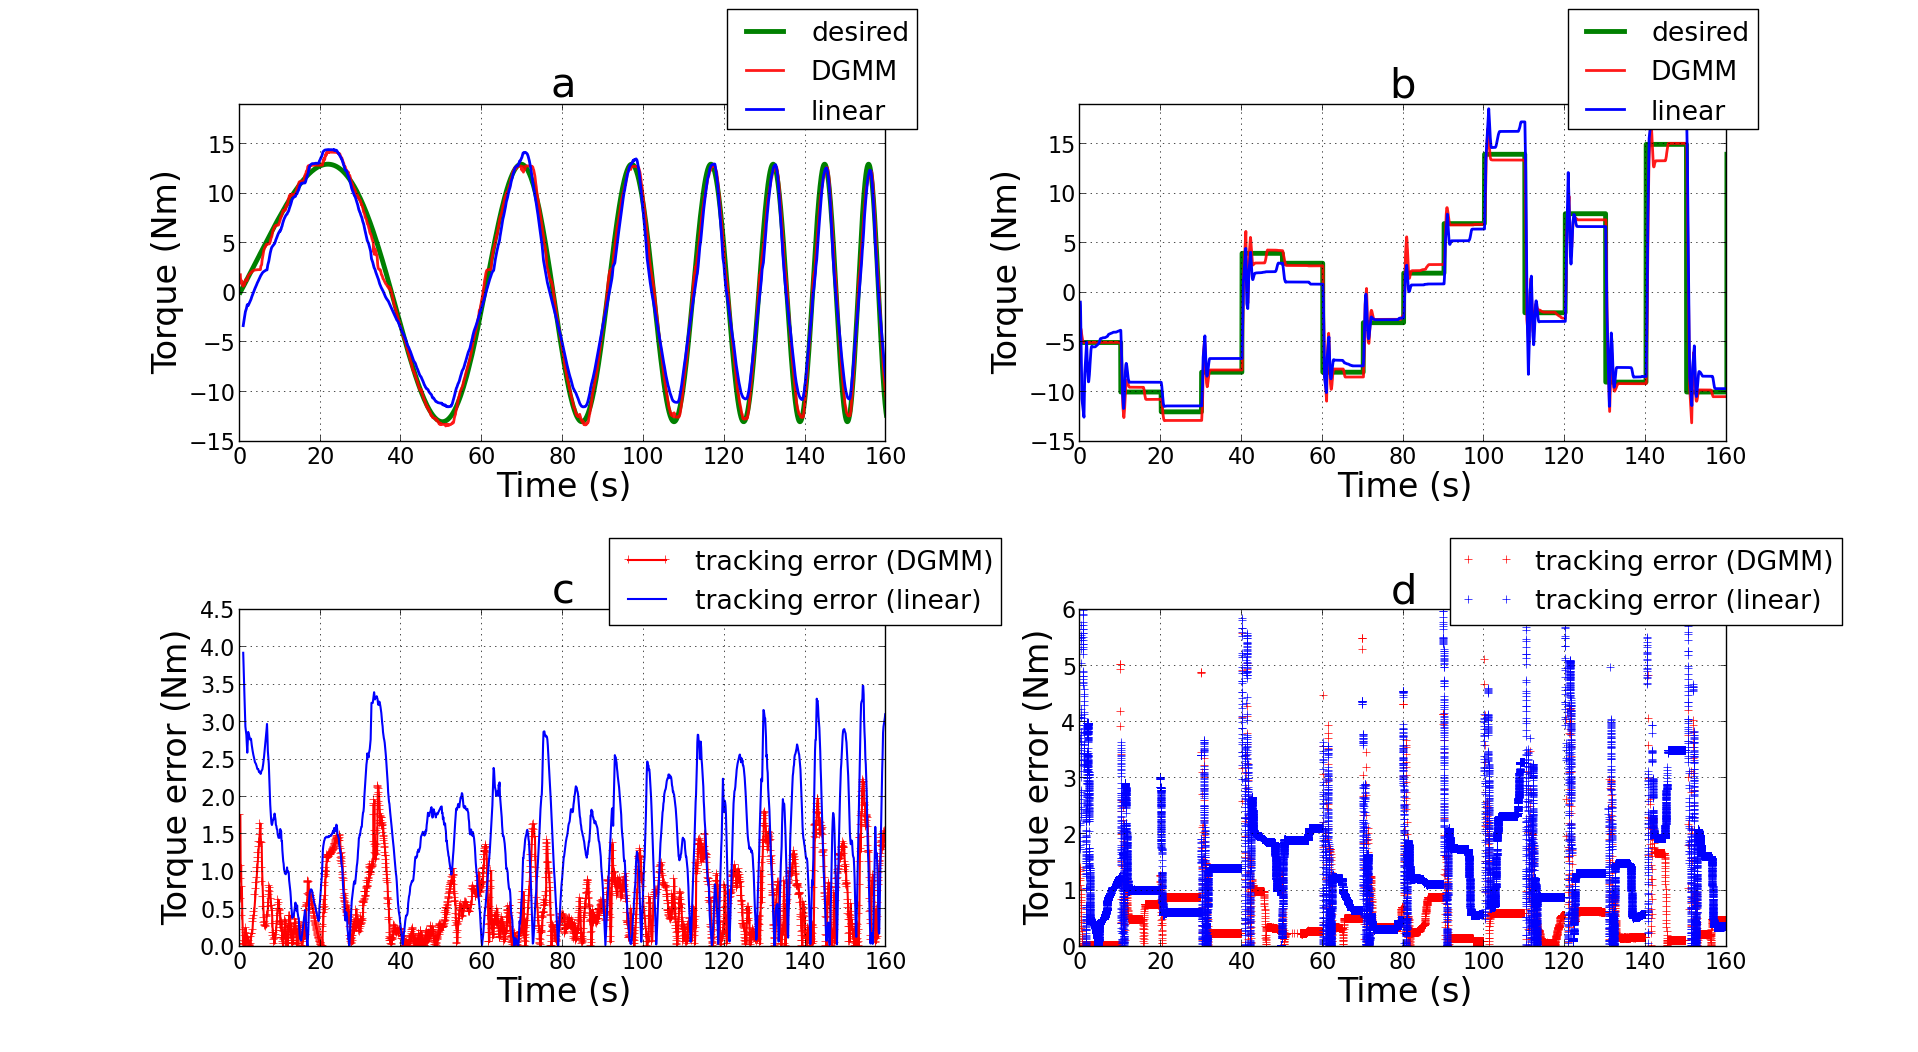
\includegraphics[width=1.15\columnwidth]{./images/4by3_torquetrack_chirp_rdwalk_comparison.png}
 \caption{\textit{a:} Result of the torque tracking with a chirp reference signal, \textit{b:} Result of the torque tracking with a random walk reference signal, \textit{c:} Torque tracking error with given chirp reference, \textit{d:} Torque tracking error with given random walk reference, }
 \label{fig:torque_tracking_result}
\end{figure}
%%%%%%%%%%%%%%%%%%%%%%%%%%%%%%%%%%%%%%%%%%%%%%%%%%%%%%%%%%%%%%%%%%%%%%%%%%%%%%






\iffalse
%%%%%%%%%%%%%%%%%%%%  Figure: torque tracking    %%%%%%%%%%%%%%%%%%%%%%%%%%%%
\begin{figure}[htb]
\centering
\advance\leftskip-1.1cm
\vspace*{-1.1 cm}
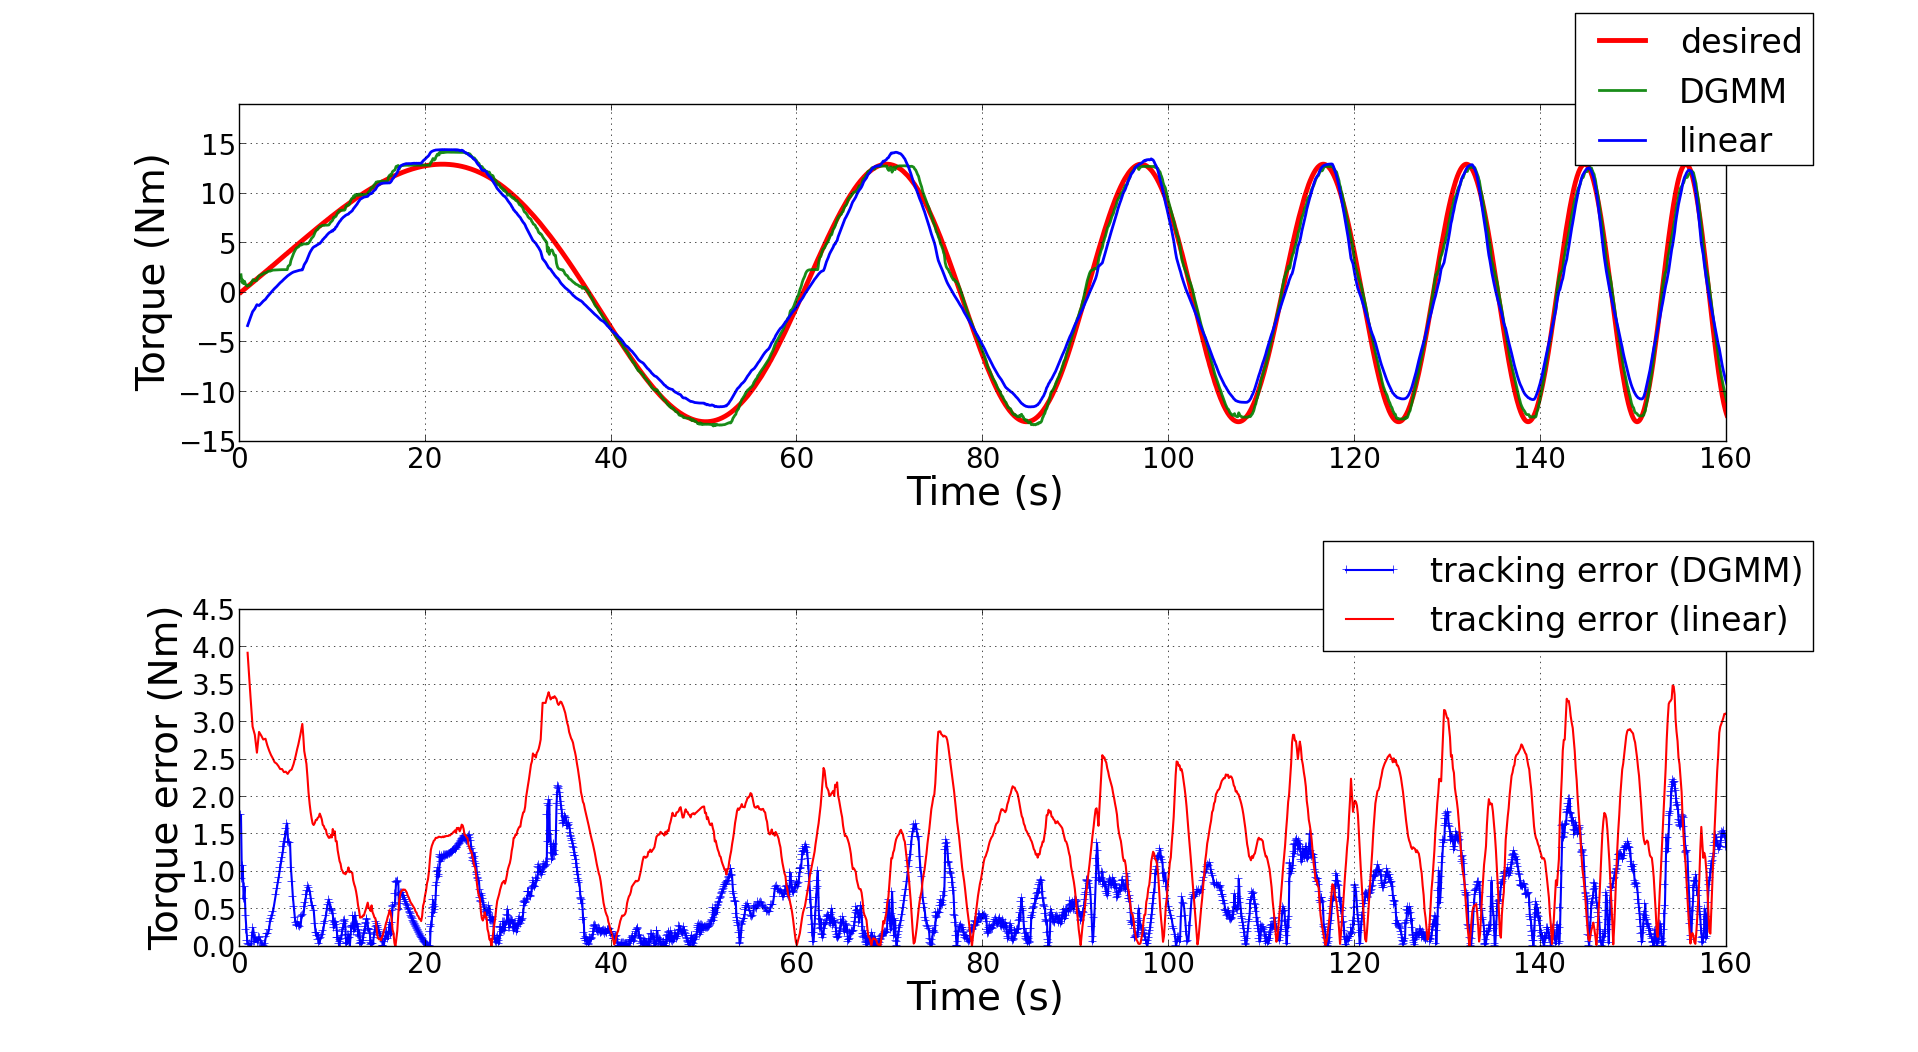
\includegraphics[width=1.15\columnwidth]{./images/4by3_dgmm_torquetrack_chirp_new.png}
 \caption{\textit{upper:} Result of the torque tracking with a chirp reference signal, \textit{lower:} Torque tracking error.}
 \label{fig:torque_tracking_result}
\end{figure}
%%%%%%%%%%%%%%%%%%%%%%%%%%%%%%%%%%%%%%%%%%%%%%%%%%%%%%%%%%%%%%%%%%%%%%%%%%%%%%

%%%%%%%%%%%%%%%%%%%%  Figure: torque tracking    %%%%%%%%%%%%%%%%%%%%%%%%%%%%
\begin{figure}[htb]
\centering
\advance\leftskip-1.1cm
\vspace*{-1.1 cm}
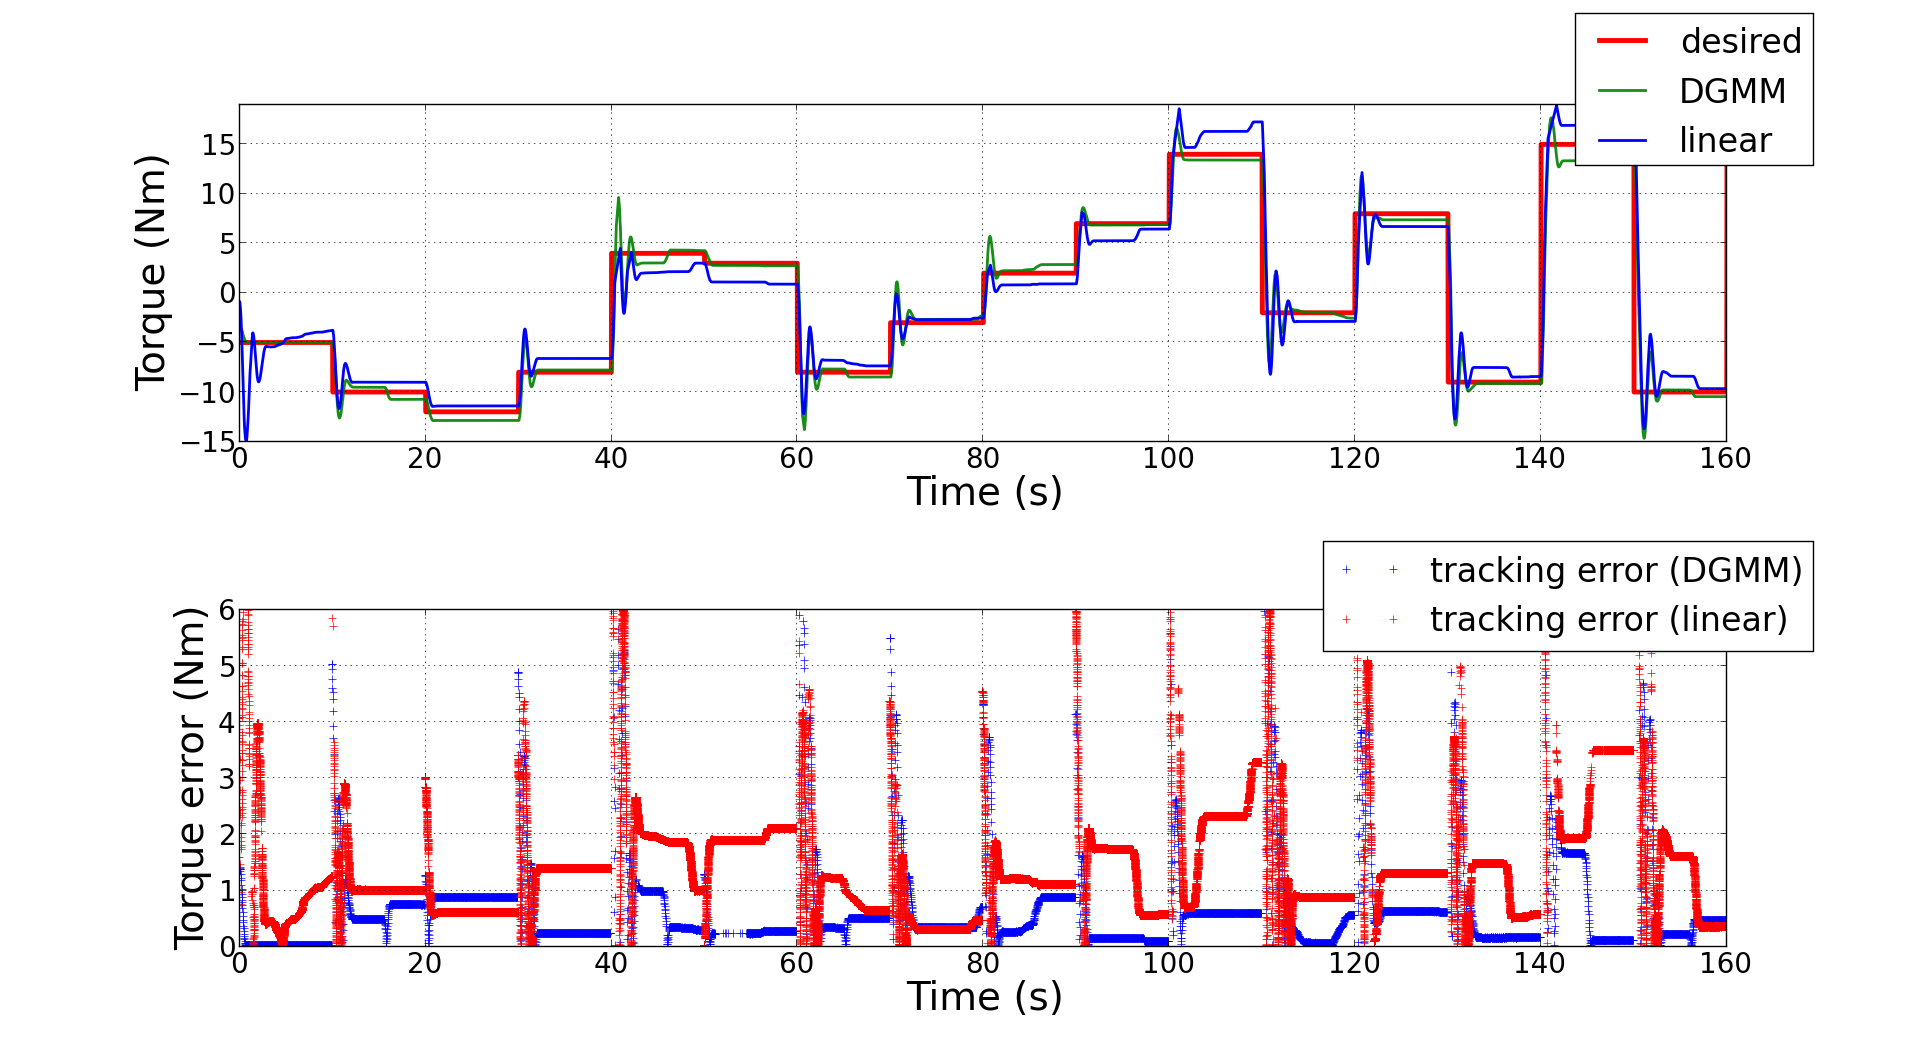
\includegraphics[width=1.15\columnwidth]{./images/4by3_dgmm_torquetrack_randomwalk_taumod.png}
 \caption{Result of torque tracking with a random-walk reference signal.}% \info{}}
 \label{fig:torque_tracking_result}
\end{figure}
%%%%%%%%%%%%%%%%%%%%%%%%%%%%%%%%%%%%%%%%%%%%%%%%%%%%%%%%%%%%%%%%%%%%%%%%%%%%%%
%Virtual Spring Element
%Gravity Compensation
%Zero Torque on Spring(Torque Control of High Compliant Series Elastic Actuator )
\fi

\section{Conclusion}
\label{sec:Conclusion}
In this paper, two data-driven modeling methods are proposed to account for the nonlinearities of the spring coupling of a rotary elastic actuator. The models are learned from the training experiments of the actuator and verified by estimating the output torque with given measured variables in the test experiments. The experiment result presents a comparable performances of the DGMM and the deep learning/NN methods, which show a significant advantage compared to a linear regression model. As compared to the DGMM model, the deep learning model shows a slight improvement in torque estimation. On the other side, the DGMM model captures multiple relationship among the observed variables, which is more flexible to be utilized once learned in multiple ways by choosing which variables are used as inputs and which ones as outputs of the model.

The learned nonlinear spring model is then used as an torque estimation module for a torque controller, which cascades with  an inner motor current and deflection control loops. The proposed torque controller is verified by a set of experiments which demonstrated a precise torque control. 
% in a short term.... in a long term... (future work).
% implement the deep learning weights in FPGA.
% improve the torque control structure. (bandwidth)
%\todo[inline]{\normalsize conclusion will be added.}%\newline}
%\listoftodos[Notes]


\begin{thebibliography}{4}
%1
\bibitem{Rollinson2013} Rollinson, D., Ford, S., Brown, B., Choset, H.: DESIGN AND MODELING OF A SERIES ELASTIC ELEMENT FOR SNAKE ROBOTS. In: Proceedings of the ASME 2013 Dynamic Systems and Control Conference, (2013)
%rubber spring

\bibitem{Paskarbeit2013} Paskarbeit, J., Annunziata, S., Basa, D., Schneider, A.: A self-contained, elastic joint drive for robotics applications based on a sensorized elastomer coupling—Design and identification, In: Sensors and Actuators A: Physical, vol. 199, pp. 56--66. Springer, Heidelberg (2013)
% elastomo

\bibitem{Edgington2009} Edgington, M., Kassahun, Y., Kirchner, F.: Dynamic motion modelling for legged robots. In: 2009 IEEE/RSJ International Conference on Intelligent Robots and Systems, pp. 4688--4694 (2009)

\bibitem{Bishop1995} Bishop, C. M. Neural networks for pattern recognition. Oxford university press. (1995)


\bibitem{Keras} Keras: Deep Learning library for Theano and TensorFlow, \url{https://keras.io/}

\bibitem{Yu2013} Yu, H., Huang, S., Thakor, N.V., Chen, G., Toh, S.L.: A novel compact compliant actuator design for rehabilitation robots. In: 2013 IEEE international conference on rehabilitation robotics,(2013)
%June 24-26 Seattle washington usa

\bibitem{Rethink} Rethink Robotics, \url{www.rethinkrobotics.com}

\bibitem{Bargsten2016} Bargsten, V., de Gea Fern\'andez, J.: COMPI: Development of a 6-DOF compliant robot arm for human-robot cooperation In: In Proceedings of the 8th International Workshop on Human-Friendly Robotics, (2015)

\bibitem{Paine2014} Paine, N., Oh, S., Sentis, L.: Design and Control Considerations for High-Performance Series Elastic Actuators. In: IEEE/ASME TRANSACTIONS ON MECHATRONICS, vol.19, no.3, (2014)
%survey of spring design, UT-SEA

\bibitem{Pratt1995} Pratt, G.A., Williamson, M.M.: Series Elastic Actuators. In: IEEE  International  Conference  on  Intelligent  Robots  and  Systems, vol.1, pp. 399--406, (1995)

\bibitem{Arumugom2009} Arumugom, S., Muthuraman, S., Ponselvan, V.: Modeling and application of series elastic actuators for force control multi legged robots. In: Journal of computing, vol.1,(2009)
%ISSUE 1, Dec, ISSN: 2151-9617

\bibitem{Kong2012} Kong, K., Bae, J., Tomizuka, M.: A Compact Rotary Series Elastic Actuator for Human Assistive Systems In: IEEE/ASME Transations of Mechatronics,vol.17,no.2,(2012)
%No.2

\bibitem{Stienen2010} Stienen, A.H.A., Hekman, E.E.G., Braak, H., Aalsma, A.M.M., Van der Helm, F.C.T., van der Kooij, H.: Design of a Rotational Hydroelastic Actuator for a Powered Exoskeleton for Upper Limb Rehabilitation. In: IEEE transactions on biomedical engineering, vol.57, no.3,(2010)

\bibitem{Mallwitz:2015} Mallwitz, M., Will, N., Teiwes, J., Kirchner, E.A.: The {CAPIO} Active Upper Body Exoskeleton and its Application for Teleoperation. In: Proceedings of the 13th Symposium on Advanced Space Technologies in Robotics and Automation. ESA/Estec Symposium on Advanced Space Technologies in Robotics and Automation (ASTRA-2015), 2015

\bibitem{Sudano2014} Sudano, A., Tagliamonte, N.L, Accoto, D., Guglielmelli, E.: A Resonant Parallel Elastic Actuator for Biorobotic Applications. In: 2014 IEEE/RSJ International Conference on Intelligent Robots and Systems (IROS), (2014)

\bibitem{Wyeth2008} Wyeth, G.: Demonstrating the Safety and Performance of a Velocity Sourced Series Elastic Actuator  In: 2008 IEEE International Conference on Robotics and Automation,(2008)

\bibitem{Li2015} Li, Y., Feng, H.: Force control of series elastic acutator In: 2015 Fifth International Conference on Instrumentation and Measurement, Computer, Communication and Control, (2015)

\bibitem{Ford2014} Ford, S., Rollinson, D., Willig, A., Choset, H.: Online Calibration of a Compact Series Elastic Actuator In: 2014 American Control Conference (2014)

\bibitem{Lu2015} Lu, C., Mao,Y., Zhu, Q., Xiong, R.: Novel series elastic actuator design and velocity control In: Electric Machines and Control, vol.19, pp.83--88, (2015)

\bibitem{Jose2016} de Gea Fern\'andez, J.,  Sprengel, H., Mallwitz, M., Zipper, M., Yu, B., Bargsten, V.: Designing Modular Series-Elastic Actuators for Safe Human-Robot Collaboration in Industrial Settings. In: Proceedings of the Climbing and Walking Robots and Support Technologies for Mobile Machines (CLAWAR),(2016)

\bibitem{Zenzes2016} Zenzes, M., Kampmann, P., Stark, T., Schilling, M.: {NDLC}om: Simple Protocol for Heterogeneous Embedded Communication Networks, In: Proceedings of the Embedded World Exhibition and Conference, at Embedded World 2016 (2016)

%\bibitem{Parietti2011} Parietti, F., Baud-Bovy, G., Gatti, E., Riener, R., Guzzella, L., Vallery, H.: Series Viscoelastic Actuators Can Match Human Force Perception. In: IEEE/ASME TRANSACTIONS ON MECHATRONICS, vol. 16, 5 (2011)
%visco-elastic model

%\bibitem{Austin2015} Austin, J., Schepelmann, A., Geyer, H.:Control and Evaluation of Series Elastic Actuators with Nonlinear Rubber Springs. In: 2015 IEEE/RSJ International Conference on Intelligent Robots and Systems, (2015)

%\bibitem{Vallery2007} Vallery, H., Ekkelenkamp, N., van der Kooij, H., Buss, M.: Passive and Accurate Torque Control of Series Elastic Actuators. In: Proceedings of the 2007 IEEE/RSJ International Conference on Intelligent Robots and Systems,(2007)
%survey of torque control with SEA

%\bibitem{Bingbin2014} Yu, B., Tibebu, A., Kassahun, Y., Bernhard, F., B. Vander Poorten, E. :Towards learning-based catheter distal section steering. In: Proceedings of the 4rd Joint Workshop on New Technologies for Computer/Robot Assisted Surgery (CRAS), pp. 167--170(2014)

%\bibitem{Yu2015} Yu, H., Huang, S., Pan, Y., Zhao,G.:Huma-robot interaction control of rehabilitation robots with series elastic actuators. In: 2013 IEEE international conference on rehabilitation robotics,(2015)

%\bibitem{Kong2009} Kong, K., Bae, J., Tomizuka, M.: Control of Rotary Series Elastic Actuator for Ideal Force-Mode Actuation in Human–Robot Interaction Applications In: IEEE/ASME Transations of Mechatronics,vol.14,no.1,(2009)

%\bibitem{Thummel2001} Th{\"u}mmel, M., Otter, M., Bals, J.: Control of Robots with Elastic Joints based on Automatic Generation of Inverse Dynamics Models In: proceedings of the 2001 IEEE/RSJ International Conference on Intelligent Robots and Systems, (2001)

\end{thebibliography}
\end{document}











































